%!!!!!!!!!!!!!!!!!!!!!!!!!!!!!!!!!!!!!!!!!!!!!!!!!!!!!!!!!!!!!!!!!!!!!!!!!!!!!!
%!NOTE: This example file has been prepared according to the University of
%!      Hawaii Style & Policy Manual for Theses and Dissertations dated
%!      "Revised September 2010". If you have one with a later date, you may
%!      need to make revisions to this document as well. In any event, making
%!      sure your thesis complies with Graduate Education guidelines is
%!      ultimately your responsibility. Caveat LaTeXtor. :)
%!!!!!!!!!!!!!!!!!!!!!!!!!!!!!!!!!!!!!!!!!!!!!!!!!!!!!!!!!!!!!!!!!!!!!!!!!!!!!!

%% The options are (you can only choose one from each group):
%%
%% 10pt, 11pt, 12pt: chooses the point size for the document. "11pt" is the
%%                   default.
%%
%% oneside, twoside: whether you want your document onesided or twosided. Note
%%                   that twosided is not guaranteed to work, and style
%%                   guidelines prohibit double sided printouts on final
%%                   copy. "oneside" is the default.
%%
%% draft, final: when printing drafts you can save a lot of paper by using the
%%               "draft" option. It switches to single spacing, displays overful
%%               hboxes with a black box, prints a version number on title page 
%%               and omits signature page. Of course for the final copy make
%%               sure to use the "final" option! "final" is the default.
%%
%% thesis, dissertation: switches between the style for a master's thesis and a 
%%                       Ph.D. dissertation. The differences are fairly minor
%%                       and limited to the front matter. "thesis" is the
%%                       default.
%%
%% actual, proposal: switches between actual document and proposal mode. In
%%                   proposal mode: the title page is simplified and the
%%                   version number is always printed.
%%
%%% Load the new uhthesis document class
\documentclass[11pt]{uhthesis}

%%% Load some useful packages:
%% New LaTeX2e graphics support
\usepackage{graphicx}
\usepackage{csvsimple}
\usepackage{longtable}
\usepackage{booktabs}
%% Package to linebreak URLs in a sane manner.
\usepackage{subcaption}
\usepackage{caption}
\usepackage{url}
\usepackage{color}
\usepackage{graphicx}
\usepackage{siunitx}
\usepackage{pgfplotstable}
\usepackage{graphics}
% Setup siunitx:
\sisetup{
  round-mode          = places, % Rounds numbers
  round-precision     = 2, % to 2 places
}
\newcommand{\hilight}[1]{\colorbox{yellow}{#1}}
%%% Declarations for Front Matter. Capitalize all of these values
%%% "normally". This allows the document class to format them properly.
%% Full title of thesis or dissertation, capitalized like a title should be.
\title{The Development of a Body Composition Imaging System Using 3D Depth Sensors Utilizing Machine Learning For Testing in Microgravity Simulations}
%% Your name, capitalized normally. Do not include any titles like Dr.
\author{Michael Omori}
%% Month in which you intend to receive your degree (i.e. graduation).
%% Presumably this will be one of: May, August, or December.
\degreemonth{May}
%% Year of expected graduation.
\degreeyear{2020}
%% Type of degree to be conferred.
\degree{Master of Science}
%% This is the chairperson of your committee. Do not use titles like Dr.
%%\chair{John Shepherd}
%% The other members of your committee, seperated by "\\". Again, no titles,
%% and it is customary to list the outside committee member (if you have one)
%% last.
\othermembers{John Shepherd, Co-Chairperson\\Peter Sadowski, Co-Chairperson\\
Kyungim Baek}
%% The field in which you are obtaining your degree, capitalized normally.
\field{Computer Science}
%% If your discipline allows subfields, you can add it here. Note that this
%% is strictly controlled, so consult the Style & Policy guide before adding
%% a subfield.
%\subfield{Bioinformatics}
%% 4-6 optional keywords/phrases for use in indexing or as search terms
%%\keywords{theses, dissertations, graduating, computer science, body composition, machine learning}
%% The version number of your document. Consistent use of this will enable you
%% to tell old drafts from new ones. Final actual documents omit this
%% automatically so you can use it without fear of submission problems at the
%% end. If you do not define this parameter, it defaults to "1.0.0".
\versionnum{4.0.0}

%%% End of preamble
\begin{document}
\maketitle

\begin{frontmatter}

%%% Note, there is no longer a signature page included in the document, it
%%% has been replaced by Form IV

%%% Create the copyright page (optional)
\copyrightpage

%%% Bring in the dedication page from external file (optional)
%%%%%%%%%%%%%%%%%%%%%%%%%%%%%%%%% -*- Mode: Latex -*- %%%%%%%%%%%%%%%%%%%%%%%%%%%%
%% uhtest-dedication.tex -- 
%% Author          : Robert Brewer
%% Created On      : Fri Oct  2 16:29:01 1998
%% Last Modified By: Robert Brewer
%% Last Modified On: Fri Oct  2 16:29:20 1998
%% RCS: $Id: uhtest-dedication.tex,v 1.1 1998/10/06 02:07:25 rbrewer Exp $
%%%%%%%%%%%%%%%%%%%%%%%%%%%%%%%%%%%%%%%%%%%%%%%%%%%%%%%%%%%%%%%%%%%%%%%%%%%%%%%
%%   Copyright (C) 1998 Robert Brewer
%%%%%%%%%%%%%%%%%%%%%%%%%%%%%%%%%%%%%%%%%%%%%%%%%%%%%%%%%%%%%%%%%%%%%%%%%%%%%%%
%% 

\begin{dedication}
\null\vfil
{\large
\begin{center}
To those in need,\\\vspace{12pt}
Those with or destined for cancer,\\\vspace{12pt}
and the group.
\end{center}}
\vfil\null
\end{dedication}


%%% Bring in the acknowledgments section from external file (optional)
%%%%%%%%%%%%%%%%%%%%%%%%%%%%%%%%% -*- Mode: Latex -*- %%%%%%%%%%%%%%%%%%%%%%%%%%%%
%% uhtest-acknowledgements.tex -- 
%% Author          : Robert Brewer
%% Created On      : Fri Oct  2 16:29:43 1998
%% Last Modified By: Robert Brewer
%% Last Modified On: Fri Oct  2 16:29:52 1998
%% RCS: $Id: uhtest-acknowledgements.tex,v 1.1 1998/10/06 02:06:54 rbrewer Exp $
%%%%%%%%%%%%%%%%%%%%%%%%%%%%%%%%%%%%%%%%%%%%%%%%%%%%%%%%%%%%%%%%%%%%%%%%%%%%%%%
%%   Copyright (C) 1998 Robert Brewer
%%%%%%%%%%%%%%%%%%%%%%%%%%%%%%%%%%%%%%%%%%%%%%%%%%%%%%%%%%%%%%%%%%%%%%%%%%%%%%%
%% 

\begin{acknowledgments}
I want to thank my committee for their guidance and feedback and give a huge thanks to all the members of the Shepherd Research Lab for making this possible (alphabetical order): Bennett Ng, Breck Yunits, Devon Cataldi, Dustin Valdez, En Yong Liu, Geraldine Ragsac, Jonathan Bennett, Laarni Igawa, Lambert Leong, Leila Kazemi, Michael Wong, Nisa Kelly, Shane Spencer, Stephanie Rania, Steven Buchthal, Thomas Wolfgruber, and Xun Zhu.
\end{acknowledgments}


%%% Bring in the abstract section from external file
%%%%%%%%%%%%%%%%%%%%%%%%%%%%%% -*- Mode: Latex -*- %%%%%%%%%%%%%%%%%%%%%%%%%%%%
%% uhtest-abstract.tex -- 
%% Author          : Robert Brewer
%% Created On      : Fri Oct  2 16:30:18 1998
%% Last Modified By: Robert Brewer
%% Last Modified On: Fri Oct  2 16:30:25 1998
%% RCS: $Id: uhtest-abstract.tex,v 1.1 1998/10/06 02:06:30 rbrewer Exp $
%%%%%%%%%%%%%%%%%%%%%%%%%%%%%%%%%%%%%%%%%%%%%%%%%%%%%%%%%%%%%%%%%%%%%%%%%%%%%%%
%%   Copyright (C) 1998 Robert Brewer
%%%%%%%%%%%%%%%%%%%%%%%%%%%%%%%%%%%%%%%%%%%%%%%%%%%%%%%%%%%%%%%%%%%%%%%%%%%%%%%
%% 

\begin{abstract}
There are several key components of health, which can be monitored through means of body composition
and shape analysis. Metrics such as fat mass index and fat free mass index are simple features of the humany body that can aid our understanding in their overall health. How these are measured have been extensively studied throughout the years. Means such as DXA and bioimpedance can accurately measure body fat. While more recently, 3d imaging has proven to be able to match the performance of its predecessors whilst providing certain benefits such as lower cost. The Shepherd Lab has demonstrated such findings by showing similar results between DXA and 3d imaging. The project is ongoing and this thesisis is the culmination of my progress relating to 3d imaging methods and testing for applications in space. It provides an overview of my work and the starting point of much future effort.

A brief overview of this work includes sensor testing, imaging configuration, a parabolic flight setup, microgravity simulation protocols, and improving the measurment of health metrics through both performance and speed. I show the importance of settings such as frame rate, resolution, and noise. Of which, the d435 sensor performs the best. With regards to the imaging configuration, I show these settings in use and the impact on the resulting 3d reconstruction. I create a system that can be used on a parabolic flight. And I also train several models for learning body fat using a graph neural network, extreme gradient boosted decision trees, and show results for the first deep learning automated caesar dataset landmark placement.

\end{abstract}


%%% Generate table of contents
\tableofcontents

%%% Generate list of tables
\listoftables

%%% Generate list of figures
\listoffigures

\end{frontmatter}

%\normalsize
%%% Bring in the body of the thesis from external file
%%%%%%%%%%%%%%%%%%%%%%%%%%%%%% -*- Mode: Latex -*- %%%%%%%%%%%%%%%%%%%%%%%%%%%%
%% uhtest-body.tex -- 
%% Author          : Robert Brewer
%% Created On      : Fri Oct  2 16:30:37 1998
%% Last Modified By: Robert Brewer
%% Last Modified On: Mon Oct  5 16:01:29 1998
%% RCS: $Id: uhtest-body.tex,v 1.1 1998/10/06 02:07:14 rbrewer Exp $
%%%%%%%%%%%%%%%%%%%%%%%%%%%%%%%%%%%%%%%%%%%%%%%%%%%%%%%%%%%%%%%%%%%%%%%%%%%%%%%
%%   Copyright (C) 1998 Robert Brewer
%%%%%%%%%%%%%%%%%%%%%%%%%%%%%%%%%%%%%%%%%%%%%%%%%%%%%%%%%%%%%%%%%%%%%%%%%%%%%%%
%% 


\chapter{Introduction}

Long duration space flights induce loss of muscle and bone mass, which in turn leads to greater risks of injury and death. To capture such changes, body composition measures are traditionally measured through Dual-energy X-ray absorptiometry (DXA); however, this is not as feasible in space. 3D optical (3DO) imaging has been demonstrated to be able to capture body composition as well as DXA, while also being hypothesized to be more easily deployable in space because of its low power consumption, higher mobility, and retainment of accuracy. We have accurate terrestrial models and the main goal of this study is to demonstrate the feasibility of our system to capture body composition in space. 
\section{Ways of getting body composition}
Dual-energy x-ray absorptiometry (DXA) is commonly used to measure bone density by measuring the abosrption of soft tissue and bone using dual x rays \cite{albanese2003clinical}. The radiation used is considered lower than normal; however, they should still be minimized in their usage which is why one would not want to take these every single day for example both for thealth impacts and costs. Due to it's versatility, DXA can also be used for total body composition and fat content measurement.

Body composition comprises of fat, bone, water, and muscle percentage. In what is known as the four compartment model \cite{fuller1992four}:
\begin{equation}
	\frac{1}{D_b} = \frac{w}{D_w} + \frac{f}{D_f} + \frac{p}{D_p} + \frac{m}{D_m}
\end{equation}
Db: overall body density, w: proportion of water, f: proportion of fat, p:proportion of protein, m: proportion of mineral, Dw: density of water, Df: density of fat, Dp: density of protein, Dm: density of mineral

Bio-electrical impedance (BIA) is used to measure volumnes, shape, or tissue electrical properties using a the general formula \cite{jaffrin2008body}:
\begin{equation}
	Z = \frac{\rho L}{A}
\end{equation}
$\rho$ is the resistance which is a metric of the tissue. L is the distance between the electrodes placed on the body. A is the area. Z is the impedance. By placing an electrode on the person's right hand and foot and sending a current through the body one measures the voltage and current with respect to time on each electrode and can determine body water and subsequently body fat. Fat and bone have higher resistance than fluid and electrolytes and thus the electrons travel differently through these mediums.

In this work, I concentrate on using imaging which has certain advantages including being non-invasive and relatively inexpensive, along with being portable.
\section{Sensor Types}
In regards to the sensors there are two main types, stereo cameras and time of flight. Along with ones such as lidar. The ideal imaging equipment roots its foundation on the attunement to the capture and reconstruction of precise depth measurements. The sensor so called, to include various imaging
modalities such as time of flight and cameras, is required to be lightweight because it needs to be
mounted. It must meet basic requirements including frame rate, resolution, precision of
acquisition, field of view. The ideal specifications surround image quality and noise. Basic hardware feature that directly affect image quality as such are pixel size and depth reconstruction algorithms. For depth, there
are a few important things. The Z-accuracy, which is the depth data accuracy. The fill rate which
evaluates the percentage of the depth coverage of the image. The RMS error which evaluates the
spatial noise or spatial depth uniformity. And the temporal noise which evaluates the temporal
uniformity over sequential frames. Other traits between sensors are mostly comparable and
company provided specs are reasonably reliable.

ToF is super-fast and the accuracy of depth is very good, but it usually suffers due to this in resolution, but they are more susceptible to light. It can be considered a type of lidar, scanner less. Time of flight uses the phase shift of amplitude modulated wave to measure the distance, while stereo is taking two pictures of the scene at different positions and generallly uses epipolar geometry. The depth depends on the reconstruction algorithm. Intel camera also have an optional infra-red used for feature matching in low contrast settings. One such way of calculating the depth from time of flight based on a simplified ideal model.

\begin{equation}
c = \lambda * f
\end{equation}
Where c is the speed of light, $\lambda$ is the wavelength and f is the frequency
\begin{equation}
	\varphi = ArcTan(\frac{A_1 - A_3}{A_2 - A_4})
\end{equation}
Where A represents the amplitudes of the sent and received signals. $\varphi$ gives us the phase shift.

\begin{equation}
	r = \frac{\pi * d * M}{n}
\end{equation}

\begin{equation}
	d = \frac{c * \varphi}{4\pi * f}
\end{equation}
The resulting depth value.

For stereovision, usually several pre-processing steps are done. After which, epipolar geometry is usually used. In which using the pinhole model, a point on the image plane of one sensor which is converted from 3d to 2d, called perspective projection. This point is somewhere in the image plane of the other sensor along the epipolar line. Using some form of criterion, we choose from several candidates of that line such as a linear function. Using simple geometry, one can then obtain the depth values as the intrinsic and extrinsic camera parameters are known.
\section{Overall Philosophy}
To obtain the values that we want we need good input values. Then it's a matter of creating a function that maps these input values to these output values in which an error function is minimized. 
This is the general setup of learning experiments. Although a machine can automatically do parts of this pipeline. There are certain parts which we consider them incapable of doing for us as of now. The primary such first example is determining the inputs. What format should the inputs be in? Ideally we could take in all of the input of the universe but this is not the case. We must limit ourselves to some relatively finite input such as images. So these images contain values from sensors. And these sensors can be your normal camera or time of flight or lidar or whatever. Other input may include descriptive information such as categorical variables like demographics: race, gender, age, etc. There are different ways to use and combine these but it is the effort of the researchers to decide on the potential use of these as information comes with a price. In regards to stereovision, it takes in two images as inputs. And matches the features in the two images. With this matching of features, one can calculate the distance from the sensor to the features. This may be primarily considered a type of feature engineering as it is not recorded input but rather engineered on top of the input. Many groups have deemed this feature of depth as supremely useful for various applications involving 3 dimensional volumes.

Thus this work concentrates on utilizing depth data from sensors for 3d reconstruction. It is possible to go directly from the depth data to body composition without the need for feature engineering such as mesh reconstruction, caesar point placement, templating, principal component analysis, and linear regression to get to body composition and shape. One could theoretically go from depth data to body composition and shape. As such this is briefly demonstrated in this work.

This thesis is composed of several main parts. The first is the comparison of the sensors for data collection. The second is the modeling of the data. The third is data simulation, augmentation, and validation through means of distribution approximation methods such as microgravity environments. Finally, the preparation for data acquisition in one such special environments known as parabolic flights.
\section{File Formats}
Here I describe a few file formats that are in use for further clarity of this document. First is the obj file. Second is the ply file. Third is the pp file. Fourth is image data. Fifth is depth data. Starting with image data which most people are familiar with. A color image will often have 3 channels one for red, one for green, and one for blue. An image that is 720 x 480 for example is 720 pixels wide and 480 pixels high. An image will contain 720 x 480 x 3 values. Depending on the acquisition format, there may be a limit to the lower and upper bounds of these values. Commonly it is a byte, 8 bits, so from 0-255. Depth data on the other hand only has one channel usually. And the upper bound of the value is usually limited by the data type used such as a 64 bit structure. It will usually represent distance from the sensor to that point in meters. These are the primary image data. There are several different mesh formats used with the two main ones in this project being the obj and the ply file.


Beginning with the obj file, this file is a human readable format. It contains information for the position of each vertex, the UV position of texture coordinates, vertex normal, and faces. Vertices are listed in counter-clockwise order. A vertex is represented as v x y z. Vertex normals are optional because faces define them. They are represented like vn x y z. Optionally, one can specify textures with vt u v. Generally a face will be defined as f v1 v2 v3. The one main requirement for an obj is the vertices. When opening this in a viewer, one can see the points. Many computer graphics, 3d printing and game rendering engines also require the face information to connect the dots along with texture information for how the faces look. In this project, only vertices and face information is used.
\begin{figure}[!htb]
	\caption{Obj File Example}
	\centering
	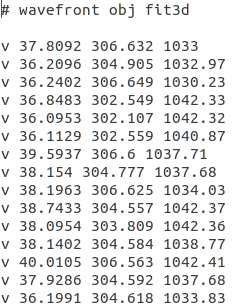
\includegraphics[width=0.3\textwidth]{images/obj_file.png}
\end{figure}
\
The ply file is similar to the obj file. There is also the option for encoding and compression of this file; otherwise the file is human readable like the obj file. A plus to this format over the obj file is the ease of adding color information. In general the file format is similar. There is the list of vertices and faces and when one wants to add color to a face one can specify a tuple such as (r, g, b) to represent the red green blue values for that face. 

\begin{figure}[!htb]
	\caption{Ply File Example}
	\centering
	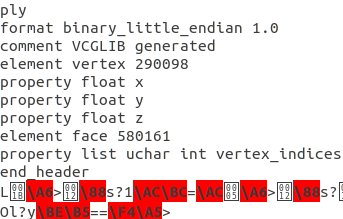
\includegraphics[width=0.3\textwidth]{images/ply_file.png}
\end{figure}
\begin{figure}[!htb]
	\caption{PP File Example}
	\centering
	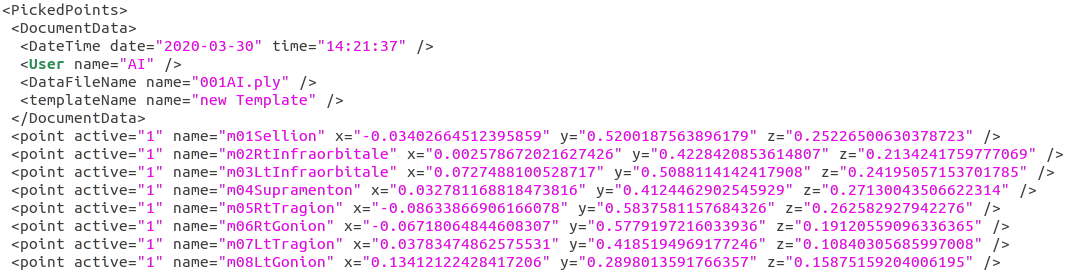
\includegraphics[width=1.1\textwidth]{images/pp_file.png}
\end{figure}

The PP file is esentially an XML format with a few components. The PickedPoints class, the document data which can contain some optional information such as : time, username, filename, and template name. Next it includes the points which in this case are for the caesar dataset. There are 75 landmarks which x, y, and z coordinates. Along with anatomical name of that point.

\section{Caesar Dataset}
The Ceasar dataset (Civillian American and European Surface Anthropometry Resource) was a project by SAE whence they collected data on 2400 US and Canadians and 2000 Europeans. 75 landmarks were taken on each of them, 3d model scans, traditional 1d measurements done with a tape measure and caliper. They include demographic information of their participants who range from ages 18-65. The 75 landmarks which I try to automatically find include points such as the sellion, iliocristale, metacarpal-phalangeal, dactlyion, tip of the nose, and so forth across the entire body. Why this is done is because they thought these points are indicative of key features of people which can provide pertinent information for use in various algorithms such as deforming a template mesh to a scanned mesh. Ideally, an algorithm could pick which points are important if necessary and disregard this.

\chapter{Previous Work}

Previous work on this included a variety of 3d scanning machines. 
\begin{figure}[!htb]
	\caption{Fit3d Scanner}
	\centering
	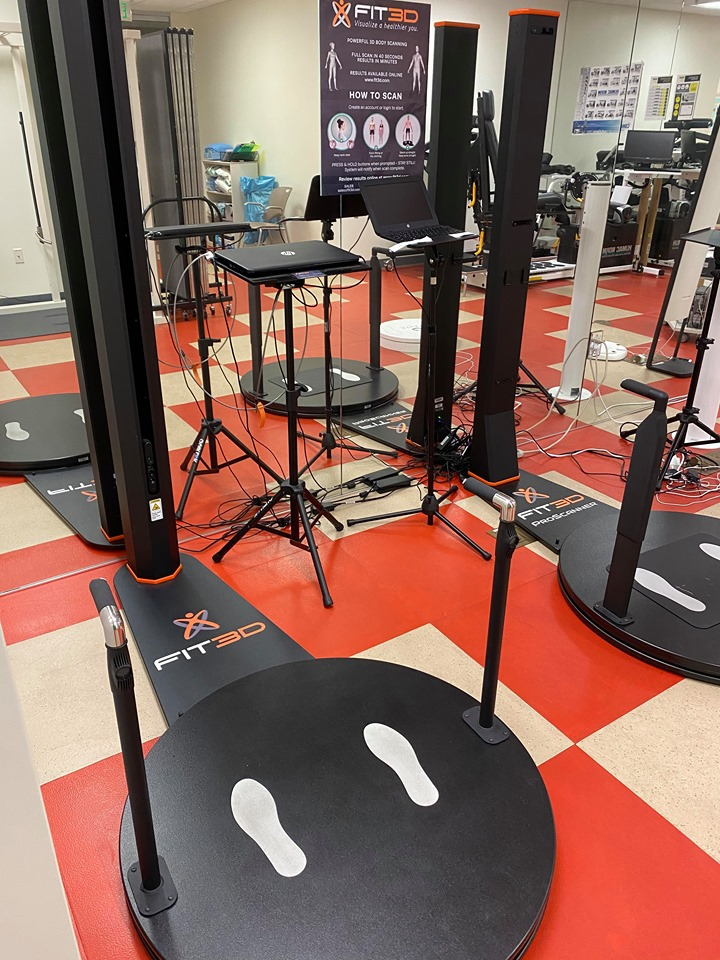
\includegraphics[width=0.5\textwidth]{images/fit3d.jpg}
\end{figure}
\begin{figure}[!htb]
	\caption{Naked Labs Scanner}
	\centering
	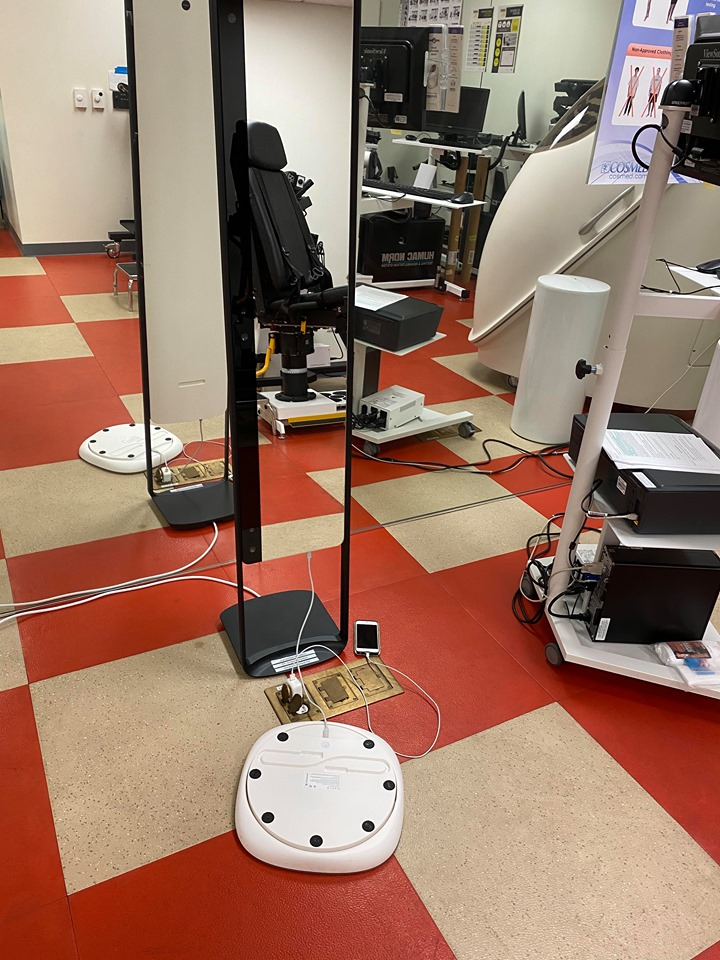
\includegraphics[width=0.5\textwidth]{images/naked_labs.jpg}
\end{figure}
\begin{figure}[!htb]
	\caption{Styku Scanner}
	\centering
	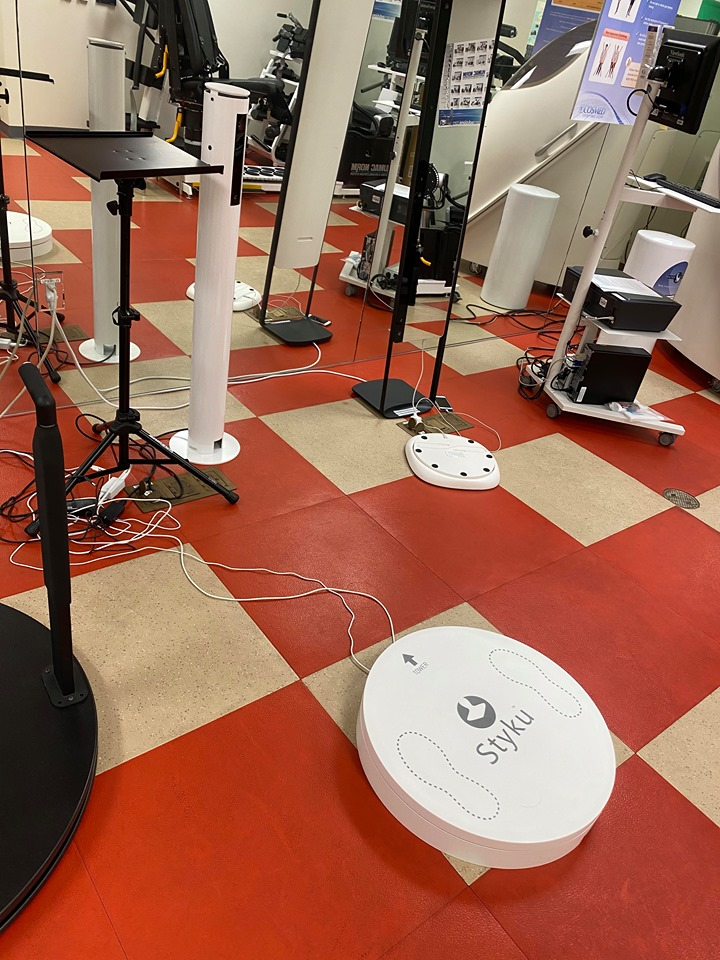
\includegraphics[width=0.5\textwidth]{images/styku.jpg}
\end{figure}
\section{3d Optical Scanners}
\begin{figure}[!htb]
	\caption{Sizestream Scanner}
	\centering
	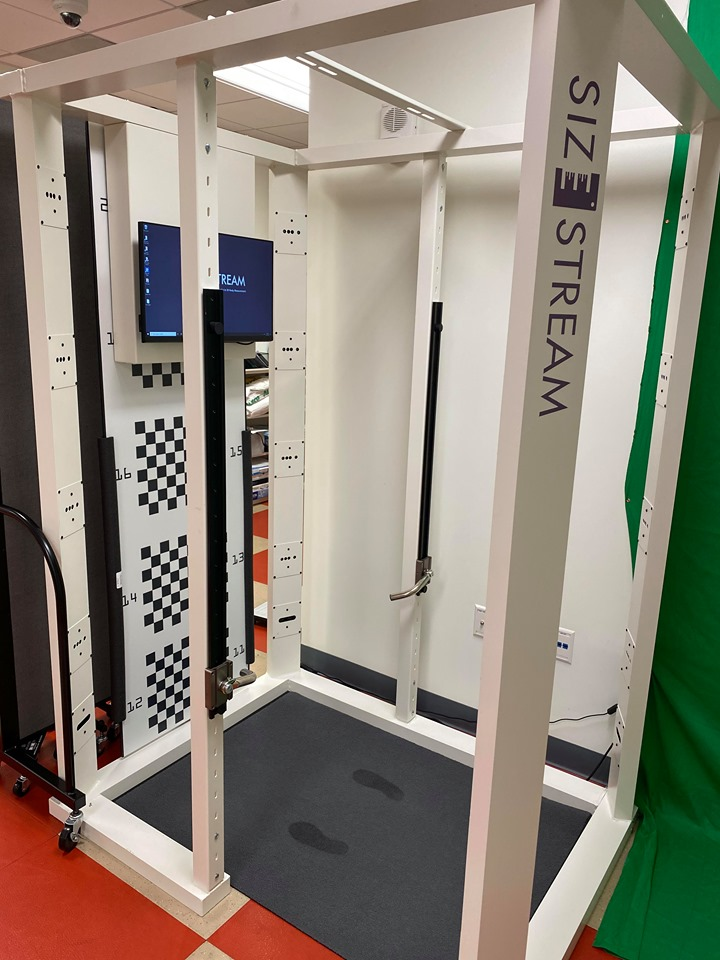
\includegraphics[width=0.5\textwidth]{images/sizestream.jpg}
\end{figure}

These scanners are all good and use a variety of kinect sensors and intel sensors.
They are good but rather inflexible in serving the purpose of imaging in space. As such, I built my own system for this. The software for these systems is not open source and depends heavily on the precise geometry of these systems. It is important to note the differentiation between these 3d optical scanners and other 3d imaging methods such as CT scans.

\section{Depth Imaging}

Next I review one of the most fundamental works on 3d imaging \cite{izadi2011kinectfusion}. KinectFusion: Real-Time Dense Surface Mapping and Tracking was a seminal work in which Microsoft developed a time of flight sensor and developed algorithms for real time reconstruction of a scene. Their method comprises of 4 main parts. Part 1 is the surface measurement, which includes the raw depth measurements along with a dense vertex map and normal pyramid map being generated. Part 2 is the sensor pose estimation which is done by predicting what the surface should be like from the previous data and using multi-scale iterative closest points to the current data. Part 3 is updating the reconstruction by fusing the current measurement with the scene model which is maintained with a truncated signed distance function. The final part is predicting the surface from part 3 which feeds back into part 2.
Further information and review of state of the art methods is given in the paper:Image-based 3D Object Reconstruction: State-of-the-Art and Trends in the Deep Learning Era \cite{DBLP:journals/corr/abs-1906-06543}.

\section{3d Reconstruction}
In 2005, Brett Allen wrote his phd thesis on learning body shape models from real-world data \cite{allen2005learning}. Both sensor technology and algorithms have come a long way since then. With a major dataset coming out of an SAE project starting in 1998. This data is not public however is the first major dataset with anthropometric measurements along with 3D stitched models from scanning of 2400 men and women.

\section{3d Neural Networks}
One of the seminal deep learning papers on 3d input was PointNet \cite{DBLP:journals/corr/QiSMG16}. It was a method used for classification and part/semantic segmentation. A couple years later, dynamic graph convolutional neural network took this further by using dynamic updates to the graph \cite{DBLP:journals/corr/abs-1801-07829}. While these methods are general, there are also more specific methods for reconstruction. A systematic approach for constructing 3d human models from 2d images \cite{5645897}. The Planck Institute published results on obtaining a mesh from a single 2d image using a combination of their previous convential method and deep learning \cite{kolotouros2019learning}.The method uses a CNN followed by their previous work SMPL and these use a self improving loop. This was tried briefly in this project. Deformable Shape Completion with Graph Convolutional Autoencoders was considered as the paper shows results on taking in an essentially partial mesh and completing it \cite{litany2018deformable}. This was put on hold though because the code is not open source and would have to be re-implemented. 

\section{Sensor testing}
Several papers have done sensor testing with depth cameras. Overall methodology was studied on these papers \cite{sophian2017evaluation} \cite{khoshelham2012accuracy} \cite{langmann2012depth} \cite{sankowski2017estimation}.


\section{Landmark prediction}
No previous paper has showed automated results on 75 points. Here is some previous work however. In Lu and Wang's work \cite{lu2008automated} they use 3d scanners and first segment the body by using silhouette analysis. Initial searches are using vertical and horizontal manual estimates. Gray-scale detection is used for identification of armpits. Following the contour of the human-body they extract more points including cervical, bust, etc, for a total of twelve landmarks. They validate on 189 subjects. In Semi-Automatic Prediction of Landmarks on Human Models in Varying Poses a Markov Network is used. The graph however is obtained manually. 200 people are used \cite{wuhrer2010semi}. Parametric body shape models were created for standing children aged 3-11 years but not adults \cite{park2015parametric}. Several models take in several depth frame data to create a shape model \cite{deng2019neural}.Lu matches the point clouds, generates a skeleton, and uses iterative linear blend skinning for learning joints \cite{lu20193d}. Stanford developed a similar idea by first registering meshes, then using a graphical model, segementation with EM to get 15 parts of a human model using the concept of rigid skeleton parts which are transformed across sequences \cite{anguelov2012recovering}.


\chapter{Methods}
There were several things I worked on. The first is a review of different sensor technologies and subsubsequent testing of the top ones. Next was the development for the Zero G Parabolic Flight which are scheduled for the summer. Third was simulating microgravity and testing them. Fourth was seeing the impact of pose on the resulting steps and final measurements.

I did a review of the sensor technologies out there excluding the commercial systems mentioned in previous works. I looked up their specs such as resolution, depth accuracy, and frame rate. I then benchmarked them on depth accuracy, temporal noise, spatial noise, and fill rate. These benchmarks were also done at varying distances. To do so, I made a simple setup. I used an imaging chart and a laser measure. I used 10 frames for each test.

\section{Graph Neural Network}
One such deep learning method that is used for 3d data inputs are graph neural networks. The one I used specifically is called dynamic graph convolutional neural network (dgcnn) \cite{DBLP:journals/corr/abs-1801-07829}. It consists of n vertices, each of which are tuple of 3 numbers. In order to apply the convolution operator, one must define an edge. With 2d images, an edge is any pixel that is adjacent to another pixel within the kernel length. For a graph, different distance metrics can be used. Dgcnn uses pairwise euclidean distances. The k nearest points are used for the subsequent convolution. Next comes the convolution kernel, which the authors define as
\begin{equation}
	E_ij = ReLU(\theta_i * (x_j - x_i) + \theta_j * x_i)
\end{equation}
Then comes max pooling for all such node j in the neighboring set of node i:
\begin{equation}
F_ij = Max(E_{ij})
\end{equation}
Before the point cloud goes into this architecture, they apply a matrix transformation using the coordinates and the differences with their neighbors.
They prove certain desirable properties such as permutation invariance and translation invariance. And achieve state of the art results on classification and segmentation in June 2019.
While they used their architecture for classification and segmentation, I convert it into regression for use in an automated caesar point placement. In Caesar, 75 landmarks are manually picked which allows a standardized template of 60k nodes to fit to the original mesh that has several hundred thousand points. Usually this takes several minutes for an expert user and can take up to an hour for a beginner.
A landmark is defined as an (x, y, z) coordinate and there are 225 such numbers that are needed to be predicted in a regression case. The other method is segmentation, which is reduced to classification of each point. In which there will be several hundred thousand points which will each need to be classified into 75 classes. Resulting in many predictions and some of these predictions may not even be exactly precise as the landmarks may not coincide directly with a point. It is hypothesized that training maybe easier in the beginning; however, in the long term one would expect a degradation in results because their is much noise. This noise comes from the fact that many points don't belong, and only 75 are really needed. With regression, one can predict the exact point and get to perfect performance. But the beginning of training may be more difficult as the predictions are totally random and the errors will be large.
The other method considered was taking in the entire mesh including face information as done by MeshCNN \cite{hanocka2019meshcnn}. It is unclear however as to the utility of face information compared to nearest neighbor information from dgcnn. As the previous information is feature extracted through non-deep learning methods in a rather arbitrary sense while neighbor information is computed by the network.

Thus for automated body shape analysis a deep learning model was briefly reoriented from dgcnn. Briefly, a deep learning model was created. 5000 scans from pca to body composition, trained on this data. PackageID from fit3d, compiled database in o drive, filename to subjectID and technology sex, height, weight, bmi, ethnicity were used. Trained to dxa values. Table 1 variables in bennets paper tied to filenames for all the scanners ask Ian were used for joins. Dxa and fit3d has 2 data points for each person, 2 values were averaged. I got a basic catboost model with the non-image features. I run a graph neural network using 1024 vertices, scaled to a unit sphere and augmented. I saved .obj files into .h5 files. .h5 file needs both data and label attributes. Numpy arrays needed to be float 32, and labels as int 64. The output is regression with multiple outputs at once using the same architecture. MSE loss caused exploding gradient thus the S was removed. File named matched to subject id and the output values. 

I also do segmentation which allows for a more pleasing visualization of the resulting mesh. It also helps reduce the output space of the network. This does add complexity to the labels as now each point needs to be labelled where previously only 75 points were labelled. Several options here include having a 76th category which is none of them. It's not clear the best way to label all the points though. Do I just take the closest point to the label and label that point and disregard the rest. I take the simplest approach algorithmically where I label all of the points to which label they are closest to. In some sense, we can compare this to label smoothing where we relax the confidence on the labels to help prevent overfitting.

\section{3d Reconstruction}
For 3d Reconstruction I use already known methods such as SPIN \cite{kolotouros2019learning} , Kinect Fusion, along with RecFusion.
\section{Sensor Comparison}

\subsection{Specs}
\begin{figure}[!htb]
	\caption{Sensor Specs}
	\centering
	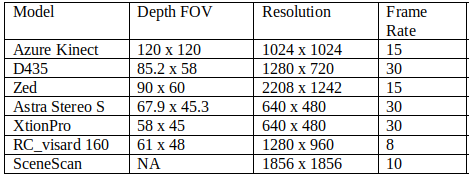
\includegraphics[width=0.7\textwidth, angle=0]{images/sensor_specs.png}
\end{figure}
I review the spec sheets for these sensors. While the above are metrics which people haven't done before on those sensors. I review depth formats such as resolution, frame rate, operating range, the color sensor corresponding features, including field of view, and where information is available online, I include the aperture, cost, sensor pixel size, software development kits (sdk).
some specs are publicly available such as these and more in depth online. It was important to us to do custom testing specific to our application in addition.

Next to calculate the approximate distance based on the field of view. We can do the following:
\begin{equation}
	Tan(\theta) = \frac{H}{2 * D}
\end{equation}
Where H is the horizontal distance of capture and D is the depth distance for capture.
\subsection{Testing Setup}
We bought and have an art easel to hold the chart. A tripod for the camera. Along with 480 LED lights 3200-5600K CRI 96+. A custom chart was bought shown in the appendix. Lights are to be positioned behind the camera at 45 degrees, with the test chart in front, figure in appendix. 
\begin{figure}[!htb]
	\caption{Sensor Testing Setup}
	\centering
	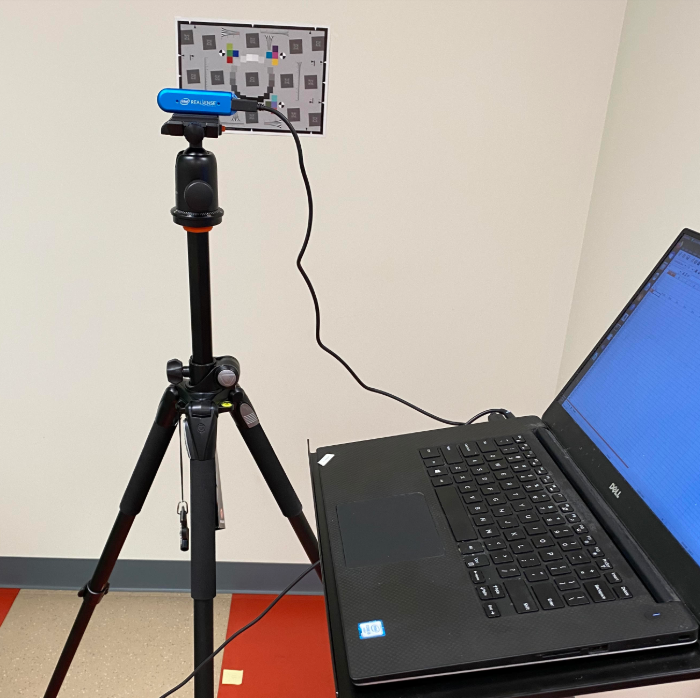
\includegraphics[width=0.5\textwidth, angle=0]{images/sensor_testing.png}
\end{figure}

\subsection{Custom Testing Metrics}
In order to choose the best sensor one could use intermediate metrics that define how good that sensor or one could use all of those sensors in the overall imaging setup and analysis and see which one works the best. The metrics I used are similar to the techincal report \cite{depthtesting}.Ideally, both should be done. I started with the first. The metrics thus defined are Z-accuracy, Fill Rate, spatial noise, and temporal noise. The Z-accuracy says how accurate the depth sensor is in relation to a ground truth(GT). We average the differences in depth sensor value and ground truth. Each metric is for a given single frame and was then average across 10 frames.
\begin{equation}
	z-accuracy = \frac{1}{n}\sum_p(Image - GT) \forall p \in box
\end{equation}
The fill rate relates to how many of the depth pixels are valid. This is useful as some sensors have high accuracy but low fill rate. This is the percentage of pixels that are non-zero.
\begin{equation}
	Fill-rate = \frac{\sum_p[I_p >= 0]}{\vert p \vert} \forall p \in box
\end{equation}
Spatial noise I define as the standard deviation divided by the mean distance.
The RMS error or spatial noise is useful to determine the x-y noise from a plane that is approximately equidistant from the imaging sensor.
\begin{equation}
	noise = \sqrt{\frac{1}{n-1}\sum_p(I_p-{\bar{I_p}})^2} \forall p \in box
\end{equation}
Last comes the temporal noise. Which is esentially the same as spatial noise except we take it across frames of the same pixel location.
\begin{equation}
	temporal-noise = \sum_p\sqrt{\frac{1}{n-1}\sum_{f=1}^{10}(I_{pf}-\bar{I_p})^2} \forall p \in box
\end{equation}
These 4 metrics are what I test. In addition to that, I compare things such as frame rate, field of view, weight, dimensions, resolution, sdks, minimum z distance and maximum z distance.

\section{Categorical Extreme Gradient Boosting}
I used Catboost \cite{DBLP:journals/corr/DorogushGGKPV17} in order to model body composition using only demographic information and was able to achieve very good performance even better than previously published \cite{article} .
\section{Parabolic Flight Setup}
The original plan was to have parabolic flights during the summer of 2020 but when we started looking into dates for zero g flights, they had regular flights then but only had research flights during the spring and fall. Thus we chose to attempt to get ready for the spring. It was a bit rushed and we almost made it, ultimately though, zero g was not able to work through some deals with other companies and coronavirus also started ramping up at that time, so the flight was postponed.
To take a 3d imaging system aboard such a flight required certain things that other people have not taken into consideration before when imaging humans for body composition. Some systems like the naked labs scanner have a mirror which encases the sensors. This is not necessary in zero g as one does not want any object to crack the mirror and the mirror is not needed for imaging. Other scanners such as the sizestream are extremely heavy and bulky and use many sensors. The height of this is larger than 60 inches which is the maximum height an object can be when brought onto the zero g flights. Thus I built my own imaging system. After testing the sensors, I selected the best one. Then tested different imaging parameters for the software such as frame rate, distance from the sensor, etc.
The figure below is what the general setup looks like.
\begin{figure}[!htb]
	\caption{Astro 3d Imaging Setup}
	\centering
	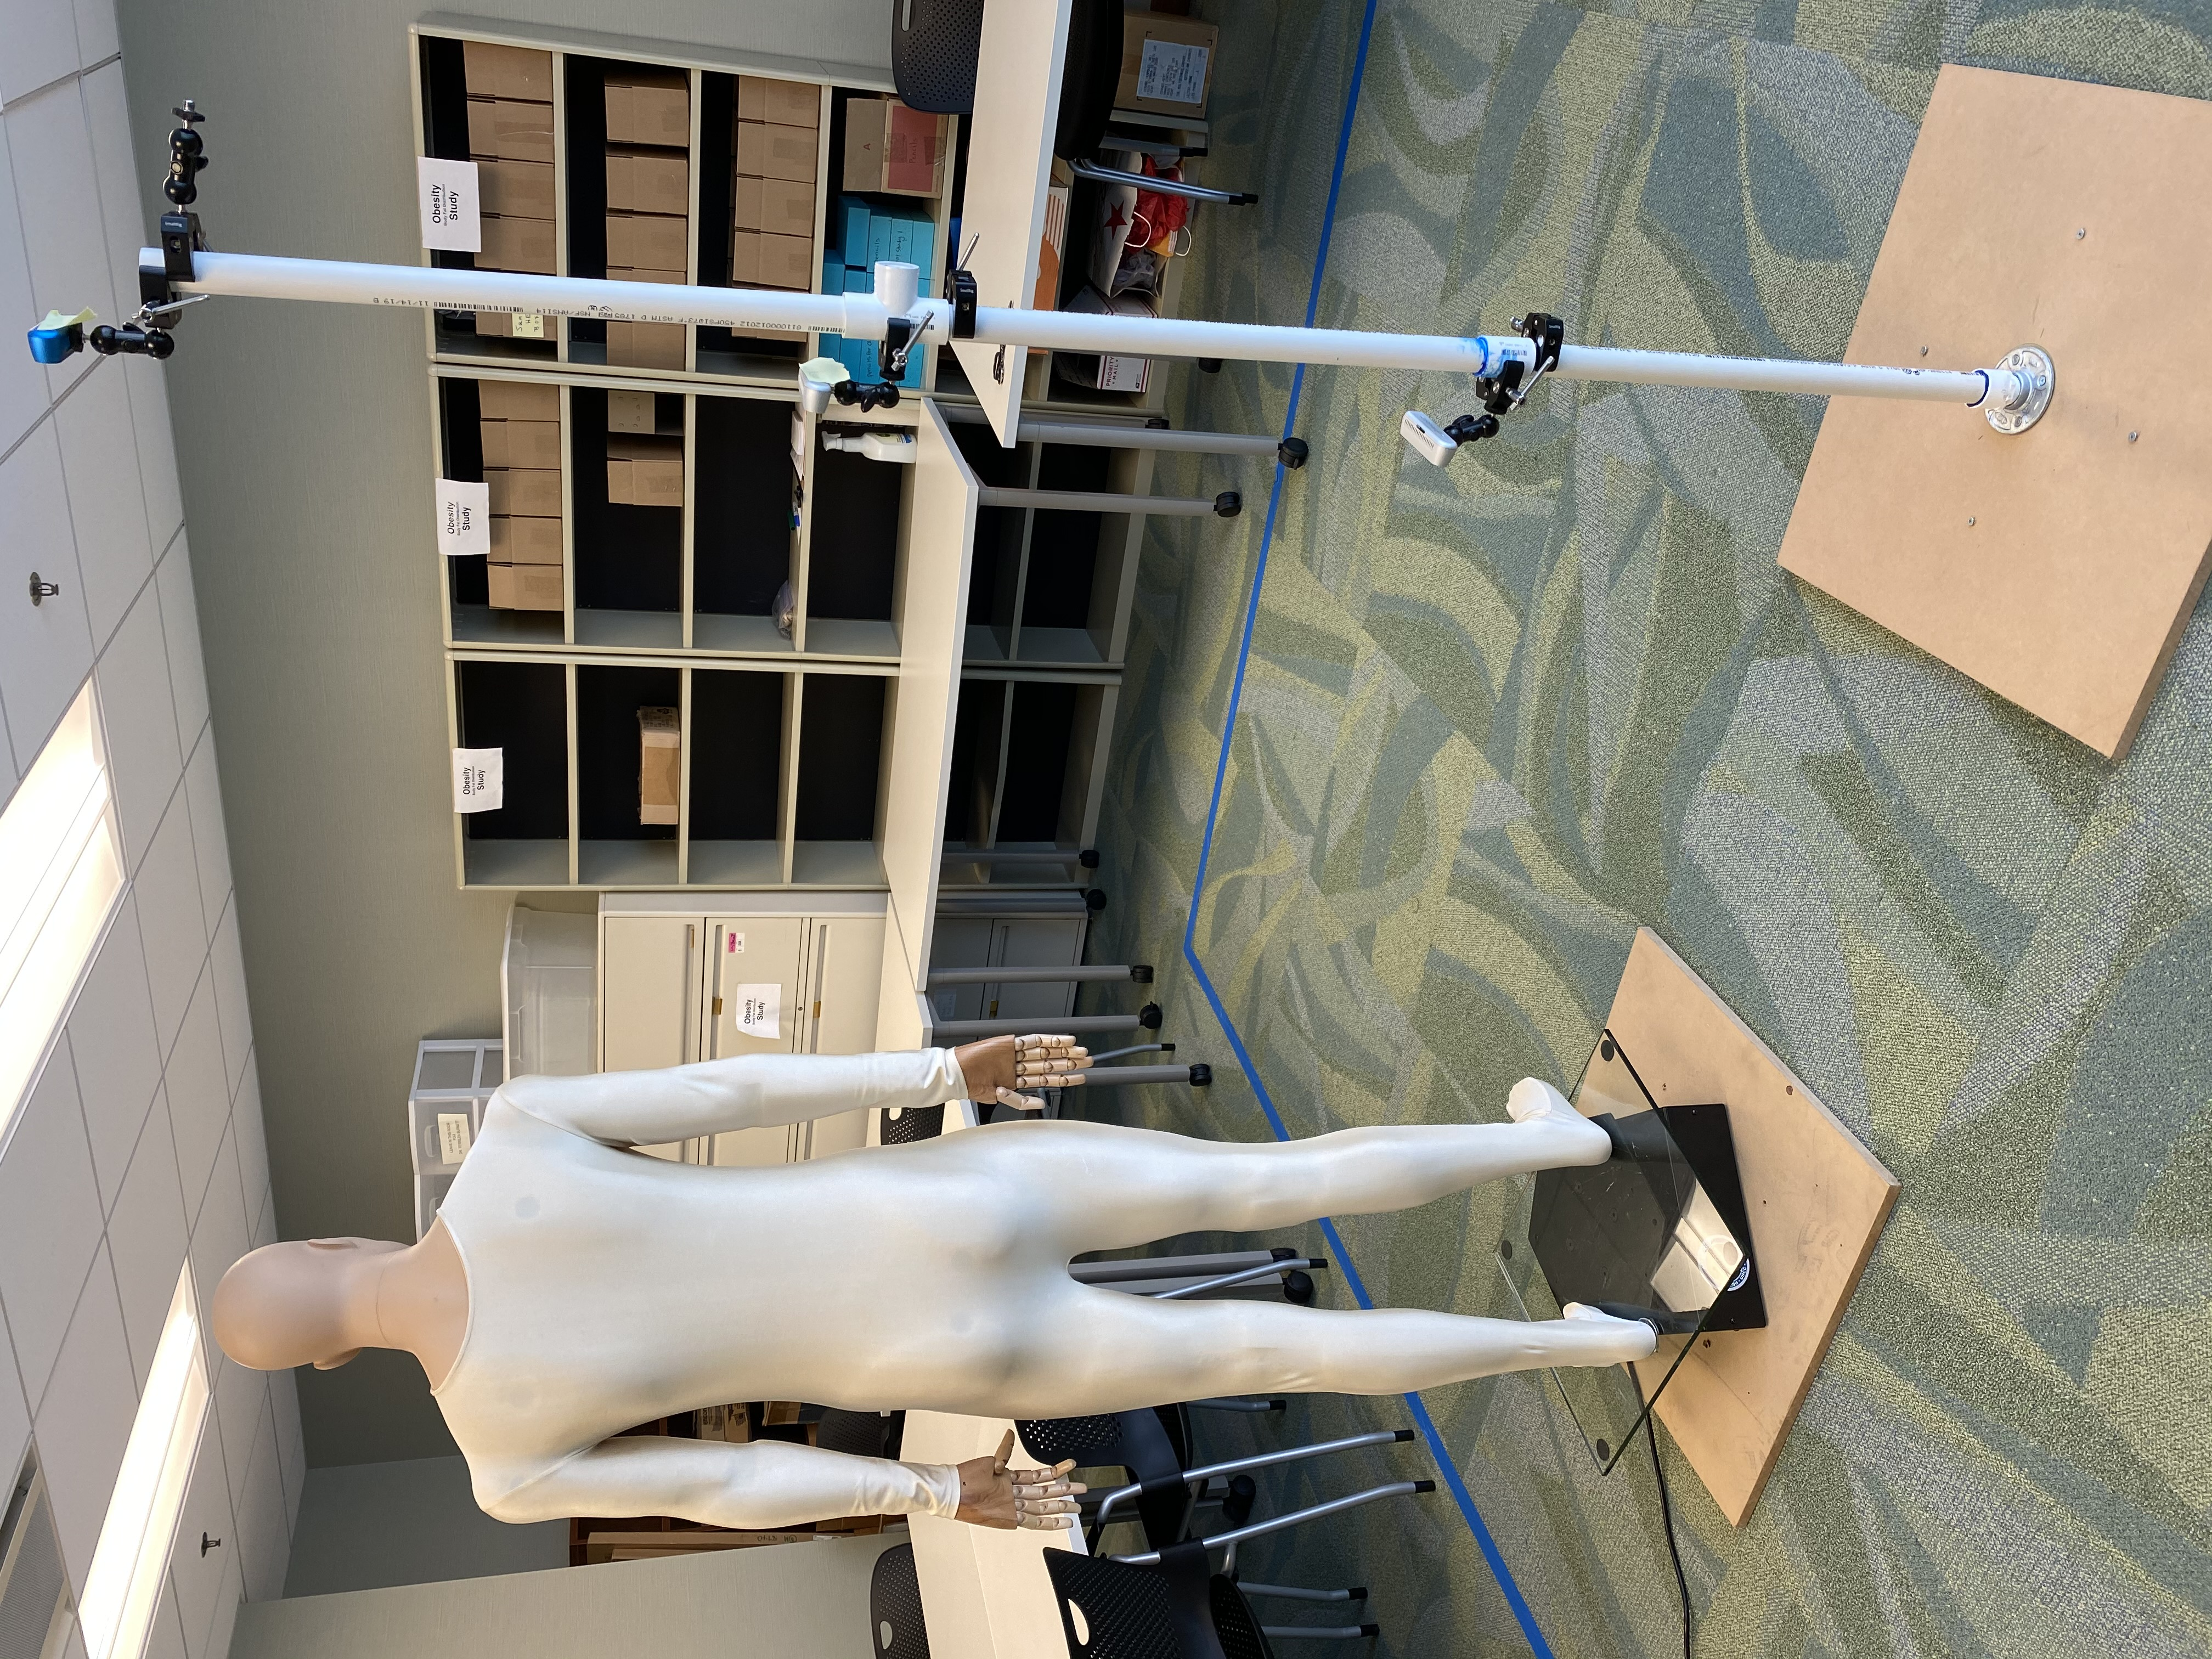
\includegraphics[width=0.7\textwidth, angle=-90]{images/astro_setup.jpg}
\end{figure}

The specific maneuver of the aircraft is ascending at \ang{45} followed by flattening the plane out followed by \ang{45} nose low fall. The G-ForceOne contains 36 seats and is 60 feet long and 10 feet wide. Due to safety concerns, the maximum height of any equipment is 60 inches. The aircraft contains attach points that are 20" x 20" (+/-1/16"). Bolt spacers are used with 3/8-24UNF threaded holes along with AN6 steel bolts for securment of equipment. Other requirements included the material be at least 1/2" thick and 24" x 24" minimum. As such, a wood board was used that is 24" x 24". This was chosen over metal because of the lessening of vibration and for ease of drilling. Strap for carrying and anchoring are used including: CGU-1/B, S0203-0338-B, and 104410P. The power type aboard to be used is 115 volts ac, 60HZ, three phase. The aircraft lighting is at 5600 kelvin and are LEDs, suitable for general photography and this type of imaging. On-board tools are properly labeled and to be stored in a toolbox. Before flight, a test readiness review is required.
The specific parts that were used are as follows 1 inch diameter steel flange for attachment of the pole to the platform. The pole used is metal for the parabolic flight and pvc for adjustable lengths on ground. Screws were used to attached the flange to the platform. 4 holes were drilled into the platform for attachment to the plane floor using AN6 steel bolts. A tight plastic cap was attached the top opening of the pole to soften any physical impact. Threaded clamps were used to attach the sensors to the pole at adjustable positions.

\section{Creating The Ideal Imaging Setup On Plane vs On Ground}
There are a few differences with the ideal imaging setup on plane vs on ground. One such being timing. As each parabolic arc is limited to only 8-15 seconds of microgravity. So we only could shoot for 8 seconds at max to be safe. While on the ground, time is only a concern due to funding for the subject's time and their availability. Thus when choosing the best parameters on ground. I tested various setups. This included sensor type, frame rate, sensor height, rotation speed, laser power, minimizing laser interference. A lot of the results are included in the appendix.
\section{Body Imaging on Babies}
Body imaging on babies is difficult because babies have trouble standing on their own. So typically they are imaged lying down. A result of this is the backside can not get imaged. The method we tried using to get a mesh of babies was a technique called SMIL\cite{hesse2018learning}. After getting it set up we got some preliminary results on fake babies that looked good. The original plan was to see how this could be used for this project too. As there are some cases where the entire body may not be able to be imgaed. This includes on an inversion table where the back is once again obscured from view of the sensors regardless of positioning. Another is the timing issue on the parabolic flights in which one could stitch together an incomplete view of the person if needed. With regards to the specifics of SMIL. We have rgb images of a baby. Depth images are in 16 and 24 bit, along with a segmented mask. The test images all have values between 791 and 957. While my images were between 0 and 255, so I added 791 to all the values. Since it was doing a cutoff at 65k, and treating the pixel values of 0 as missing. The table segmentation needs to be manually adjusted however as this affected the energy terms and subsequent mesh generation.
\section{Microgravity Simulation}


\begin{figure}[!htb]
	\caption{Inversion Table}
	\centering
	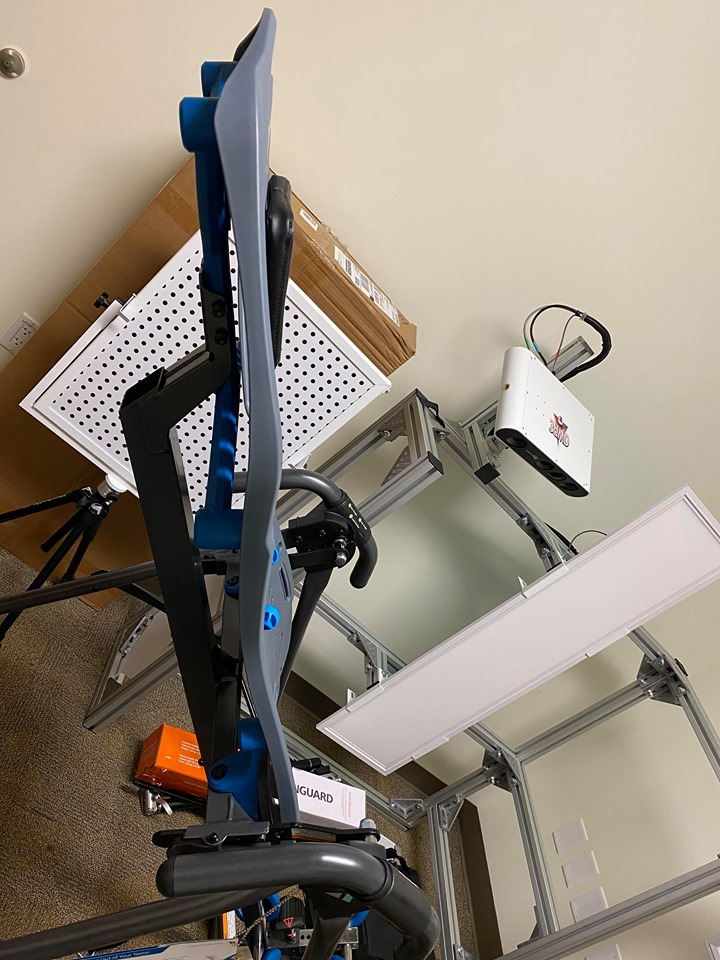
\includegraphics[width=0.5\textwidth]{images/inversion.jpg}
\end{figure}
\subsection{Underwater Imaging}
Some other ways besides parabolic flight testing to simulate microgravity include gravity boots, inversion tables, and underwater imaging. The protocols were developed for these but scanning of participants was halted due to coronavirus. Planning for underwater imaging was briefly explored. A 2016 paper by Disney research \cite{digumarti2016underwater} used intel realsense cameras and a custom capture device. They demonstrated how calibration is different underwater along with the refraction model required. With such results, one could go on to perform 3d reconstruction from this mapping. Some things that have not been before include a complete scan of human bodies underwater which may require a scanning protocol and/or multiple sensors. These are a work in progress for this project.
\subsection{Inversion Table}
Sample protocol described as follows. Different angles from -90 to about -45 degrees. Let’s say capture at intervals x. Where x is 15 degrees. Each subject will be different on the amount of time they can handle. Let’s say we want to capture 135 / x angles for y amount of minutes. We can say y is 5 minutes, where 10 minutes is extreme, while some may only be able to handle a few minutes. How much does it take for a subject to go back to baseline? Let’s say y +- e minutes, where e is 0. So to capture one angle will take 10 minutes if it’s 15 degrees, that’s 9 takes. Which is about 90 minutes. Plus some time to get in and out. We can assume about 2 hours. So 30 athletes will take 60 hours. There are of course different considerations for the angle interval x, and time interval y. The main thing depends on time constraints and subject health. The protocol could be reversed too, to see if the order of inversion has an effect. The inversion table itself is 58” x 29” x 61”. Currently one camera can be attached to the inversion table with a stick and clamp. For inversion table imaging, it would require the single sensor moving protocol. Same goes for gravity boots. 

\section{Mesh Quality}
There are various ways of ranking mesh quality. One such is using a human to rate the quality. With enough supervision, one could create a deep learning model to output mesh quality. This is quite time consuming. Another is to run each mesh through different pipelines and see how it performs on the end result for getting values such as body composition. This methodology is also good but our current methodology is not entirely automated. The method may not give the best accuracy but is completely automated in comparison to the previous approaches. There are many ways of defining similarity. One such way with text is to first perform some type of learning such as next word prediction in word2vec and then take the first feature set known as embeddings and use them as a dense representation. Upon which people have taken measures such as cosine angle similarity which can work better than euclidean distance sometimes in high dimesnional data. More advanced methods include using a neural network such as a siamese neural network which runs two pieces of text through the same network, obtains a final representation, and outputs a similarity score using a kernel function or something as previously mentioned like cosine similarity \cite{bertinetto2016fully}. The need for this in text comes from the fact that there is no precise highly correlated numerical representation for text, rather it is highly context dependent. With images, as simple way is to take a simple l1 or l2 distance at each pixel and channel. Neural networks of course can also be used again. Other methods may include using neighborhood information which can reduce the impact of outliers such as through a gaussian distribution summation. Meshes are similar in the sense they are numerically represented like images. But they are different because there is no direct correlation between vertices like that of images which are aligned by x-y position. In this case, once again, one can use a neural network and get some intermediate representation and get the similarity from there. Due to time limitations, I perform a simple method for mesh similarity. This method is used in often in the fusion of meshes and/or alighment of meshes. It is known as iterative closest point (icp).

One more well known distance metric worth mentioning is the Hausdorff distance which is a point estimate \cite{huttenlocher1993comparing}:
\begin{equation}
	d_h(X, Y) = max{sup(inf(d(x, y),sup(inf(d(x,y))}, x\in X, y\in Y
\end{equation}
Where sup is suprememum and inf is infimum.
Iterative closest points is as follows:
\begin{equation}
	E(R, t) = \frac{1}{N_p}\sum_{i=1}^{N_p}||x_i - Rp_i - t||^2
\end{equation}
$x_i$ and $p_i$ are corresponding points.
While in general, there are many performance things done for this algorithm. With t representing translation and R representing rotation. We do not have to consider these because our lack of dynamacy. Thus our problem is simplified. On top of this, I perform quadric edge collapse reduction to reduce the seach space as a form of sampling \cite{hussain2004efficient}.
The above may be considered as geometric measurments of quality, which do not correlate necessarily with human visual perception. So although I try this metric. I also try another metric, that which is the number of connected components in the graph. Where a connection between two vertices is defined as a face that includes those two vertices.

It is interesting to note many previous works include mesh quality using a refernce mesh which is tried in this. But due to large variety of pose and variance caused by configuration setup, I largely do not go with this approach. Many use the similarity of the surface of the meshes and compare them that way along with visual cues if color is of importance such as contrast.
\chapter{Results}
\section{Sensor Testing Results}
The below figure shows the spatial resolution per frame of the d435. This was done to test if the spatial noise changes with the number of frames and the distance. The number of frames does not appear to have an impact; however, the spatial noise is increasing relative to the distance after an adjustment to the distance. This suggests that the closer the sensor to the object the better. However, thereis a limit to how close these sensors can get.
\begin{figure}[!htb]
	\caption{Spatial Resolution per frame of d435}
	\centering
	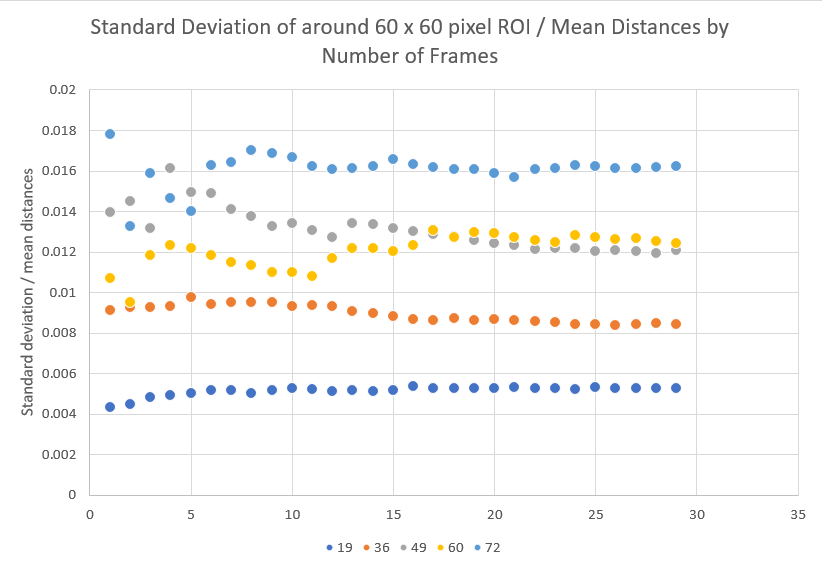
\includegraphics[width=0.7\textwidth]{images/d435_spatial_resolution.png}
\end{figure}

Here is the chart for sensor accuracy. The average errors by sensor are: 0.864 for the D435, 1.366 for the Azure Kinect, 1.739 for the D415, 2.446 for the Kinect Windows, and 2.489 for the Kinect XBOX. While these metrics are not all precise as there is some error from the human, the results shown are averaged across multiple frames to partially counteract this.
\begin{figure}[!htb]
	\caption{Sensor Accuracy by Distance}
	\centering
	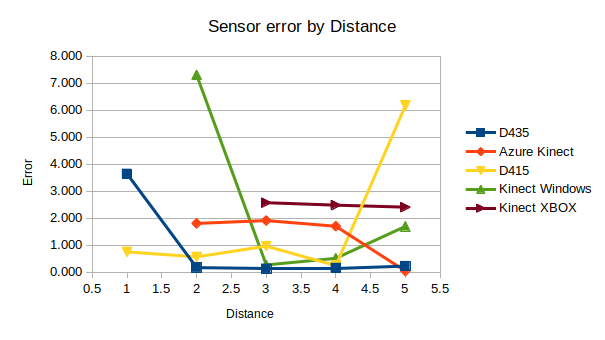
\includegraphics[width=0.7\textwidth]{images/sensor_accuracy.png}
\end{figure}

For temporal noise, the D415 scored the best in this category. This is partly explained by the d435 being like the d415 except having its sensors more spread out. The winner in this category is the Kinect Azure with an average temporal noise of 0.07 percent, then comes the kinect for windows at 0.14, kinect 360 at 0.15, d415 at 0.22, and d435 and 3.99.
\begin{figure}[!htb]
	\caption{Sensor temporal noise by distance}
	\centering
	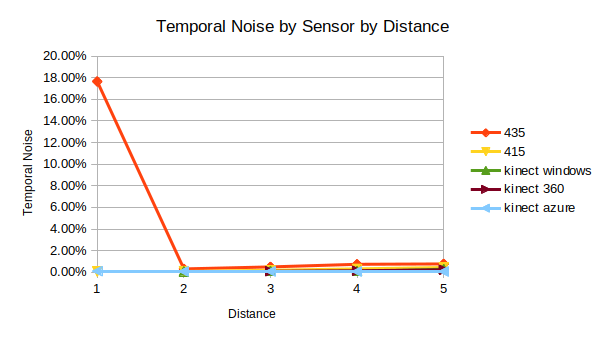
\includegraphics[width=0.7\textwidth]{images/temporal_noise.png}
\end{figure}

Fill rate, at first may not seem that important but once you look at the actual depth images you can really see the difference between the sensors. If we exclude the kinect windows because it can't take data at 1 feet away and the kinect 360 which can't take data closer than 2 feet. The best sensors are d435 at 89.86 percent, d415 at 74.81, then Azure at 70.00. The Azure Kinect makes a very interesting design choice as the developers only keep pixels that the sensor is very confident in to maintain better accuracy. While the Kinect Windows and Kinect 360 trade this off by showing more valid pixels but have a reduced accuracy. With this judgement, it is even unclear whether the Azure kinect is even a better sensor in terms of specs as if one applied this same reduction in uncertain pixels in the kinect windows and kinect 360, those sensors may achieve comparable results.

\begin{figure}[!htb]
	\caption{Fill rate of sensor by distance}
	\centering
	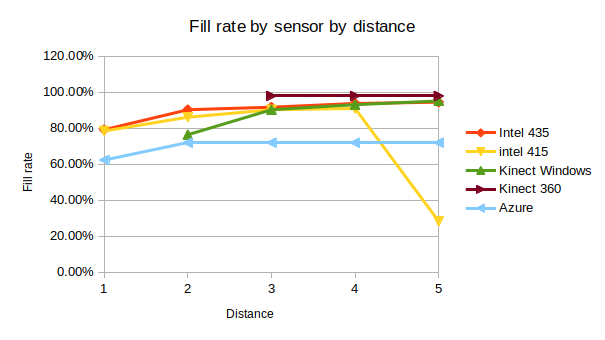
\includegraphics[width=0.7\textwidth]{images/fill_rate.png}
\end{figure}

\subsection{Sensor Specs}
The d435 is capable of reaching up to 100 frames per second which for this particular imaging application is not that useful, but an application in like drones for example, it could be more useful. One thing to note is that 100 frames per second is a lot especailly when combined with multiple sensors and a high quality data connection and cpu is needed to transfer the data fast enough. One can refer to the specs for more details and I just outline some of the main findings. The strong point of the azure kinect is it's large field of view in certain settings of \ang{120} by \ang{120}. While the d435 has a max depth resolution of 1280 x 720. The depth field of view for the d435 is \ang{85.2} horizontal and \ang{58} vertical. At first it was unclear the advantage this would bring but after testing, I realized the field of view is very useful in allowing the sensor to get closer to the target and allow the target to remain in the field of the view of the sensor. As getting as close as possible is very helpful. The azure kinect is meant for closer range solution as the operating range varies between modes but the low end is 0.25m and the high end is 5.46m. While the d435 boasts a max range of 15m, it can only get 1m close. So just comparing this, the azure kinect is preferred for this use case. Next I do a quick review of the color sensor. When I first spec'd these out, I didn't know the impact but after working with sensors and methods, the current methods primarily rely on the depth sensor information. It is only in the case of calibration in which the sensor configuration is changing that the color sensor is used to locate the physical calibration boards using color features. But when building up the mesh of the scene, is the depth sensor that is being used and the color sensor has no use currently, although it could potentially as it provides information unavailable in the depth sensor.


\section{Automated Anthropometry Results}

\begin{figure}[!htb]
	\caption{Training of Automated Caeasr Point Placement}
	\centering
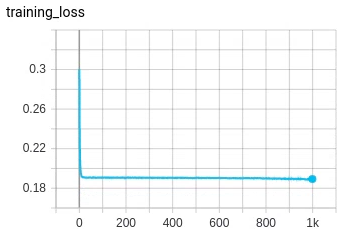
\includegraphics[width=0.5\textwidth]{images/training.png}
\end{figure}
\begin{figure}[!htb]
	\caption{Validation of Automated Caeasr Point Placement}
	\centering
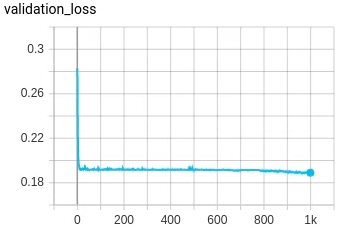
\includegraphics[width=0.5\textwidth]{images/validation.png}
\end{figure}
 \begin{figure}[!htb]
	\caption{Training of Automated Caeasr Point Placement without beginning}
	\centering
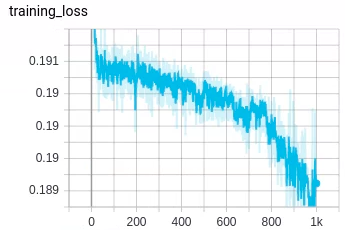
\includegraphics[width=0.5\textwidth]{images/train_close.png}
\end{figure}
\begin{figure}[!htb]
	\caption{Validation of Automated Caeasr Point Placement without beginning}
	\centering
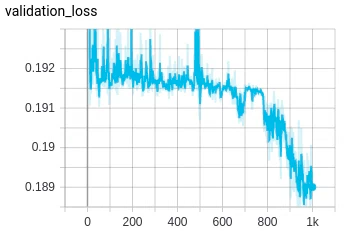
\includegraphics[width=0.5\textwidth]{images/val_close.png}
\end{figure}

We can see the training and validation errors quickly go down after about 10 epochs possibly from simply predicting the mean value of the output, then continues to go down very slowly. There is no sign of overfitting as the validation loss and training loss are similar to each other. Because only 1024 points are used, this greatly inhibits the capability of the netowrk to learn but was used for quick demonstration purposes. The number does not give me much intuition about the quality of the points. There are a couple ways to do this. One is to see how the final body shape composition results are and the other is to visualize the data. I decide to visualize the data because it could be helpful as a guide for humans if the points aren't place accurately by the algorithm  I decide to visualize the data because it could be helpful as a guide for humans if the points aren't place accurately by the algorithm. 

\begin{figure}[!htb]
	\caption{Mesh colored by labels}
	\centering
	\includegraphics[width=0.5\textwidth]{images/mesh_coloring.png}
\end{figure}

For segmentation, I frame the problem in terms of classification.

\section{Graph Neural Network and Catboost Body Composition Results}

Some basic data exploration was done like counting of missing data. Distributions of the target variables were plotted, along with the features. Using catboost, after 999 iterations, I got a test RMSE mean of 2436, std of 791, train rmse mean of 1368, std of 109. The 0th iteration was 24,584 test rmse mean, 1346 std. 24,611 train rmse mean error, 336 std. In the most recent shape up paper, it was stated that the best results were 3070 for men, and 2630 for women using 3D PC + Anthro with 5 fold CV. I also tried a graph neural network. Where the data is .obj file with vertex and face information. I removed face information and sampled the vertex information. Next, I reformulated the classification architecture for regression. I did a quick test, trained only on 10 scans, after 50 epochs had about 8000 L1 loss. I also investigated sparse autoencoders, denoising, and contrastive for dimensionality reduction in comparison with principal component analysis.


\begin{figure}[!htb]
	\caption{Fat Mass Training Table}
	\centering
	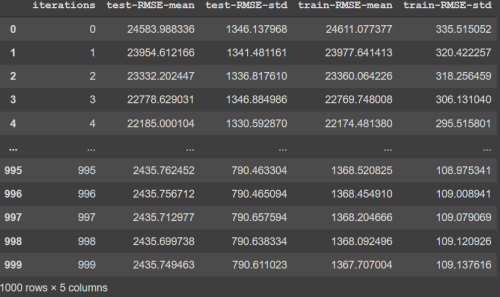
\includegraphics[width=0.9\textwidth]{images/catboost_training.png}
\end{figure}

Previous best results for RMSE on male were 3.07kg and 2.63kg for female while these results average across genders with a validation RMSE of 2.44kg. Demonstrating non-linearities in the dataset.

\section{Parabolic Setup}
The fligh was postponed. Several tries were done. Originally a multi-post base was designed. This added support but also complexity. Which is why a single pole was chosen over it. Along with this, the single pole was quite stable as the weight of the sensors is light.

\section{3d Imaging Testing Results}

\begin{figure}[!htb]
	\caption{Single d435 sensor moving imaging}
	\centering
	\includegraphics[width=0.5\textwidth]{images/dustin.png}
\end{figure}

\begin{figure}[!htb]
	\caption{Single d435 sensor moving imaging form fitting}
	\centering
	\includegraphics[width=0.5\textwidth]{images/mw_form.png}
\end{figure}



\begin{figure}[!htb]
	\caption{Mannequin imaged at 90 frames per second}
	\centering
	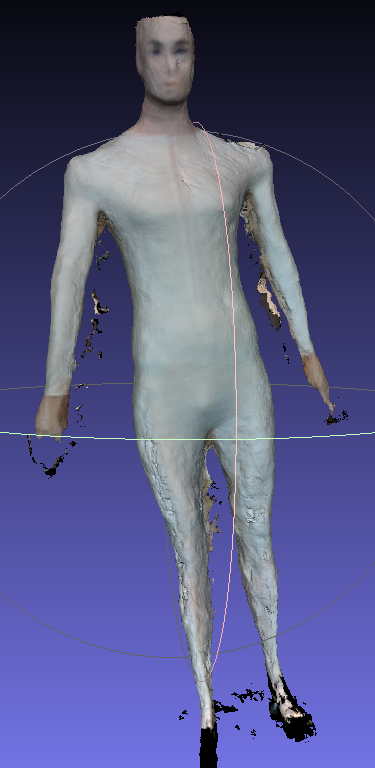
\includegraphics[width=0.2\textwidth]{images/90fps_mannequin.png}
\end{figure}


\begin{figure}[!htb]
	\caption{Mannequin imaged at 6 frames per second}
	\centering
	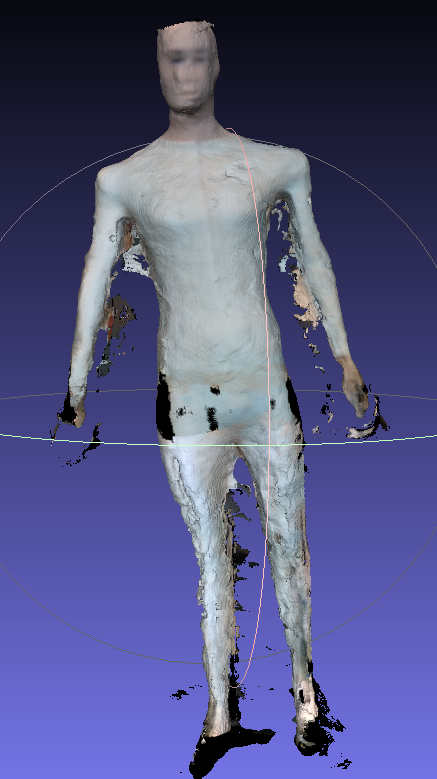
\includegraphics[width=0.2\textwidth]{images/6fps_mannequin.png}
\end{figure}

\begin{figure}[!htb]
	\caption{Mannequin imaged with a laser on and off}
	\centering
	\includegraphics[width=0.5\textwidth]{images/laser.png}
\end{figure}


\begin{figure}[!htb]
	\caption{Mannequin 90fps, 30fps, and 6fps, at full rotation speed}
	\centering
	\includegraphics[width=0.7\textwidth]{images/framing.png}
\end{figure}


\begin{figure}[!htb]
	\caption{Mannequin 100, 50, 9 percent speeds}
	\centering
	\includegraphics[width=0.7\textwidth]{images/rotation.png}
\end{figure}

\begin{figure}[!htb]
	\caption{Mannequin Depth resolution of 1280x720, 640 x 480, 480 x 270}
	\centering
	\includegraphics[width=0.7\textwidth]{images/depth_resolution.png}
\end{figure}


\begin{figure}[!htb]
	\caption{Mannequin ideal}
	\centering
	\includegraphics[width=0.7\textwidth]{images/man_ideal.png}
\end{figure}



We can see how at this setting, a higher frame rate helps with the imaging. There is more noise at 6 frames per second and it looks like the background is more part of the body because the sensor has more difficulty tracking the larger change in positioning of the mannequin.
\begin{figure}[!htb]
	\caption{Inversion Table Imaging \ang{0}, \ang{30}, \ang{60}, \ang{90}}
	\centering
	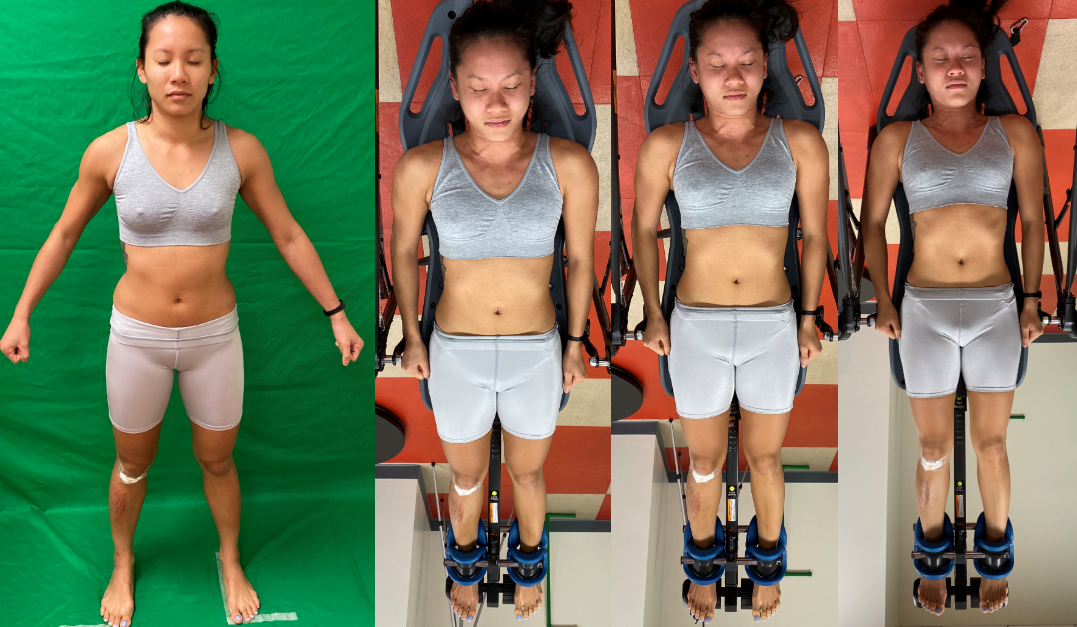
\includegraphics[width=0.7\textwidth]{images/en_inversion.png}
\end{figure}

\section{Inversion Table Imaging}

\begin{figure}[!htb]
	\caption{Inversion Table Imaging \ang{0}, \ang{30}, \ang{60}, \ang{90}}
	\centering
	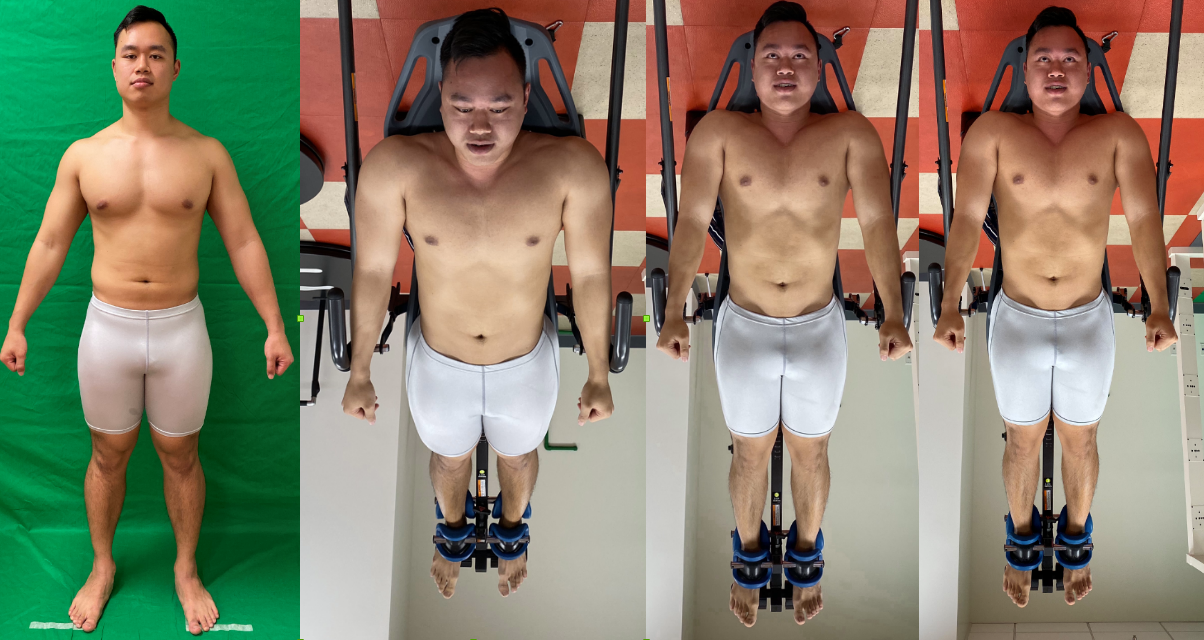
\includegraphics[width=0.7\textwidth]{images/mw_inversion.png}
\end{figure}


\section{Mannequin Imaging}
The best results for imaging come with a single moving sensor. As this sensor can capture different parts of the body more easily than when the sensors are static and the object is moving. In general frame rate helps with reconstruction especially when there is more motion of the object. This is the case when our turntable is rotating at maximum speed. It was noticed that minimizing laser interference helped with the reconstruction. This happens when multiple sensors emit infra-red, they can interact with each other. For the rotation speed of the turntable, slower is better because it makes it easier for tracking of the body. With depth resolution, higher resolution helps but is interesting to notethat this appears to taper off once the resolution reaches 640 x 480. The closest 3 sensors can get to a 6 foot person a turntable is about 3 feet because the calibration pattern needs to be seen consecutively in pairs of rgb sensors. Thus the single moving sensor is able to achieve very nice results by getting a couple feet away. Along with this, there is no need for matching each sensor up to each other, which may give some incorrect results.


\chapter{Conclusion}

I did a comparison of various 3d imaging sensors. I found that the closer the sensor to the object, the less spatial noise; however there is a certain minimum distance for each sensor that it can image.So in general one wants to get the sensor as close as possible beyond this minimum distance. The D435 had the lowest error when using a stationary target. The temporal noise for the sensors were all extremely low. Fill rate had interesting results with the Kinect 360 having the highest fill rate. While the azure kinect had the lowest fill rate. One can clearly see the poor fill rate when looking at the depth image of the azure kinect. It would seem like one of the reasons they did this was to boost the accuracy of the sensor on pixels it was sure of. While the previous kinects have these edge problems, they still reported a value regardless of its accuracy.

The graph neural network is the first method to use deep learning to automatically pick caesar points. The performance could be greatly improved with more data. Currently only about 1500 scans were used. This is because each scan also has to be human labelled with 75 points which is time consuming.

Microgravity simulation hypothetical protocols were drafted for inversion table imaging. Some inversion table imaging was done without reconstruction. The main difficulty with this is removing the table from the body.

Finally, a system to image people in parabolic flight was designed and constructed for eventual use in space by astronauts.



%%% Switch to appendix mode
\appendix

%%% Bring in any appendices from external file (optional)
%%%%%%%%%%%%%%%%%%%%%%%%%%%%%% -*- Mode: Latex -*- %%%%%%%%%%%%%%%%%%%%%%%%%%%%
%% uhtest-appendix.tex -- 
%% Author          : Robert Brewer
%% Created On      : Fri Oct  2 16:31:12 1998
%% Last Modified By: Robert Brewer
%% Last Modified On: Mon Oct  5 14:41:05 1998
%% RCS: $Id: uhtest-appendix.tex,v 1.1 1998/10/06 02:07:03 rbrewer Exp $
%%%%%%%%%%%%%%%%%%%%%%%%%%%%%%%%%%%%%%%%%%%%%%%%%%%%%%%%%%%%%%%%%%%%%%%%%%%%%%%
%%   Copyright (C) 1998 Robert Brewer
%%%%%%%%%%%%%%%%%%%%%%%%%%%%%%%%%%%%%%%%%%%%%%%%%%%%%%%%%%%%%%%%%%%%%%%%%%%%%%%
%% 

\chapter{Some Other Results}

\begin{figure}[h]
        \caption{Inversion table depth image from the intel d435 in color at a rotated view to emphasize the 3D capture and how pixels directly behind the line of sight of the sensor to object will show up as invalid dark pixels.}
        \centering
        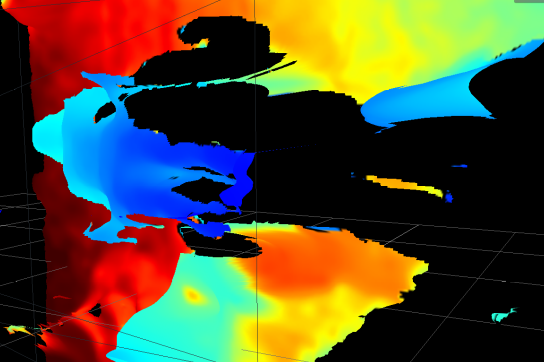
\includegraphics[width=0.5\textwidth]{images/inversion_depth.png}
\end{figure}

\begin{figure}[h]
        \caption{Three vertical sensor best setup reconstruction results}
        \centering
        \includegraphics[width=0.2\textwidth]{images/3sensor_man.png}
\end{figure}


\begin{figure}[h]
        \caption{Zero-G Cross Section}
        \centering
        \includegraphics[width=1\textwidth]{images/zerog_cross.png}
\end{figure}

\begin{figure}[h]
        \caption{Zero-G Floor}
        \centering
        \includegraphics[width=1\textwidth]{images/zerog_floor.png}
\end{figure}


\begin{figure}[h]
        \caption{Inversion table depth image from the intel d435 in color at a rotated view to emphasize the 3D capture and how pixels directly behind the line of sight of the sensor to object will show up as invalid dark pixels.}
        \centering
        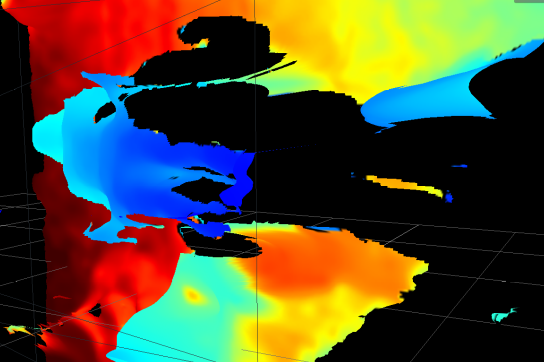
\includegraphics[width=0.5\textwidth]{images/inversion_depth.png}
\end{figure}


\begin{figure}[h]
        \caption{Sensor Testing Chart}
        \centering
        \includegraphics[width=0.5\textwidth]{images/chart_full.png}
\end{figure}
 
 
\begin{figure}[h]
        \caption{Euclidean Error vs. Depth Frame Rate show 30 and 60 frames per second as the best.}
        \centering
        \includegraphics[width=0.7\textwidth]{images/error_depth_frame.png}
\end{figure}
  
\begin{figure}[h]
        \caption{Euclidean Error vs. Rotation Rate where a high speed of 100 did the worst and bringing it down to 75 helps but then performance is about the same below that speed.}
        \centering
        \includegraphics[width=0.7\textwidth]{images/rotation_error.png}
\end{figure}
  
\begin{figure}[h]
        \caption{Euclidean Error vs. Total Depth Resolution in which the middle setting did the best.}
        \centering
        \includegraphics[width=0.7\textwidth]{images/depthres_error.png}
\end{figure}

\begin{figure}[h]
        \caption{Error vs. Total Color Resolution results show the lowest resolution as the best which hypothetically would be because higher resolution slows down the performance and color is not used for the reconstruction after calibration has been completed.}
        \centering
        \includegraphics[width=0.7\textwidth]{images/error_color.png}
\end{figure}
 

\begin{figure}[h]
        \caption{SPIN 3d reconstruction on single 2d rgb image}
        \centering
        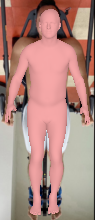
\includegraphics[width=0.2\textwidth]{images/spin.png}
\end{figure}

\begin{figure}[!htb]
        \caption{Missing data in the shape up data}
        \centering
        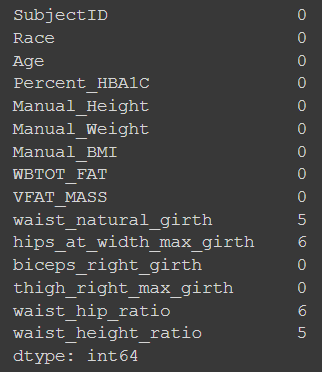
\includegraphics[]{images/missing_data.png}
\end{figure}

\begin{figure}[!htb]
        \caption{HBA1C Distribution in the shape up data}
        \centering
        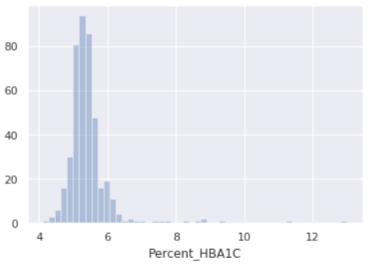
\includegraphics[width=0.5\textwidth]{images/hba1c.png}
\end{figure}

\begin{figure}[!htb]
        \caption{WBTOT FAT Distribution in the shape up data}
        \centering
        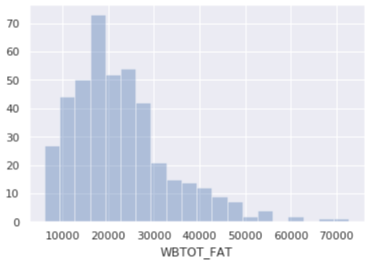
\includegraphics[width=0.5\textwidth]{images/wbtot_fat.png}
\end{figure}


\begin{figure}[!htb]
        \caption{VFAT MASS Distribution in the shapeup data}
        \centering
        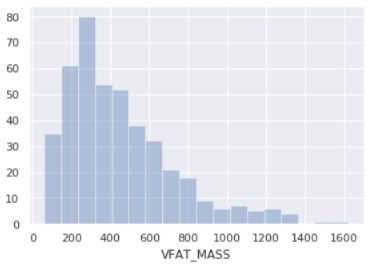
\includegraphics[width=0.5\textwidth]{images/vfat_mass.png}
\end{figure}

\begin{figure}[!htb]
        \caption{Race Ratios Distribution in the shapeup data}
        \centering
        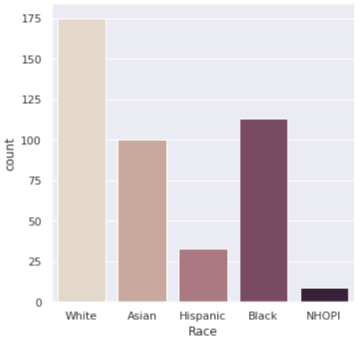
\includegraphics[width=0.5\textwidth]{images/race_ratios.png}
\end{figure}
\begin{figure}[!htb]
        \caption{Fat Mass Training Table using Catboost}
        \centering
        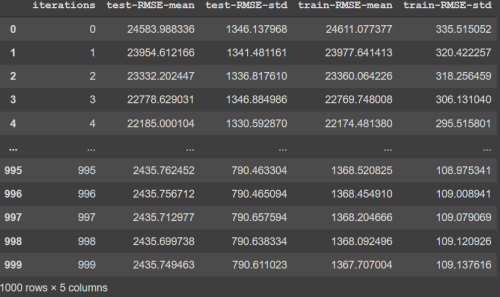
\includegraphics[width=0.7\textwidth]{images/catboost_training.png}
\end{figure}

\begin{table}[!h]
\caption{Connected Components per Experiment excluding vertical setups because of some techincal issues faced with the algorithm}
\centering
\pgfplotstabletypeset[
    col sep=comma,
    string type,
    columns/.style={column type={|l}},
    columns/.style={column type={|l}},
    every head row/.style={before row=\hline,after row=\hline},
    every last row/.style={after row=\hline},
    ]{tables/cc.csv}
\end{table}


\begin{table}[!h]
\caption{Manual and Euclidean Error Results per Experiment}
\centering
\pgfplotstabletypeset[
    col sep=comma,
    string type,
    columns/.style={column type={|l}},
    columns/.style={column type={|l}},
    columns/.style={column type={|l}},
    every head row/.style={before row=\hline,after row=\hline},
    every last row/.style={after row=\hline},
    ]{tables/manual.csv}
\end{table}

\begin{table}[!h]
\caption{Mannequin imaging table 1 partial parameters}
\centering
\pgfplotstabletypeset[
    col sep=comma,
    string type,
    columns/.style={column type={|l}},
    columns/.style={column type={|l}},
    columns/.style={column type={|l|}},
    columns/.style={column type={|l}},
    columns/.style={column type={|l}},
    columns/.style={column type={|l}},
    every head row/.style={before row=\hline,after row=\hline},
    every last row/.style={after row=\hline},
    ]{tables/test.csv}
\end{table}

\begin{table}[!h]
\caption{Mannequin imaging table 2 partial parameters}
\centering
\pgfplotstabletypeset[
    col sep=comma,
    string type,
    columns/.style={column type={|l}},
    columns/.style={column type={|l}},
    columns/.style={column type={|l|}},
    columns/.style={column type={|l}},
    every head row/.style={before row=\hline,after row=\hline},
    every last row/.style={after row=\hline},
    ]{tables/test2.csv}
\end{table}

\begin{table}[!h]
\caption{Table of Sensor Accuracy by distance to the sensor (in.)}
\centering
\pgfplotstabletypeset[
    col sep=comma,
    string type,
    columns/.style={column type={|l}},
    columns/.style={column type={|l}},
    columns/.style={column type={|l|}},
    columns/.style={column type={|l}}, 
    columns/.style={column type={|l}},
    columns/.style={column type={|l|}},
    columns/.style={column type={|l}},
    every head row/.style={before row=\hline,after row=\hline},
    every last row/.style={after row=\hline},
    ]{tables/accuracy.csv}
\end{table}
% Setup siunitx:
\sisetup{
  round-mode          = places, % Rounds numbers
  round-precision     = 2, % to 2 places
}
\begin{table}[!h]
\caption{Table of Sensor Temporal Noise by distance to the sensor (in.)}
\centering
\pgfplotstabletypeset[
    col sep=comma,
    string type,
    columns/.style={column type={|l}},
    columns/.style={column type={|l}},
    columns/.style={column type={|l|}},
    columns/.style={column type={|l}}, 
    columns/.style={column type={|l}},
    columns/.style={column type={|l|}},
    columns/.style={column type={|l}},
    every head row/.style={before row=\hline,after row=\hline},
    every last row/.style={after row=\hline},
    ]{tables/temporal-noise.csv}
\end{table}

\begin{table}[!h]
\caption{Table of Fill Rate by distance to the sensor (percent)}
\centering
\pgfplotstabletypeset[
    col sep=comma,
    string type,
    columns/.style={column type={|l}},
    columns/.style={column type={|l}},
    columns/.style={column type={|l|}},
    columns/.style={column type={|l}}, 
    columns/.style={column type={|l}},
    columns/.style={column type={|l|}},
    columns/.style={column type={|l}},
    every head row/.style={before row=\hline,after row=\hline},
    every last row/.style={after row=\hline},
    ]{tables/fill-rate.csv}
\end{table}
\begin{figure}[!htb]
        \caption{Connected Components Best Mesh}
        \centering
        \includegraphics[width=0.2\textwidth]{images/cc_best_mesh_2.png}
\end{figure}
\begin{figure}[!htb]
        \caption{Connected Components Worst  Mesh}
        \centering
        \includegraphics[width=0.2\textwidth]{images/cc_worst_mesh_6.png}
\end{figure}

\begin{figure}[!htb]
        \caption{Best mesh by euclidean distance}
        \centering
        \includegraphics[width=0.2\textwidth]{images/euclidean_ideal.png}
\end{figure}

\begin{figure}[!htb]
        \caption{A fully human labeled mesh, all 300,000 vertices colored by closest caesar landmark}
        \centering
        \includegraphics[width=0.2\textwidth]{images/full_labeled_mesh.png}
\end{figure}

\begin{figure}[!htb]
        \caption{A subsampled human caesar labeled mesh by color}
        \centering
        \includegraphics[width=0.3\textwidth]{images/labeled_mesh.png}
\end{figure}

\begin{figure}[!htb]
        \caption{Ideal mesh reposed through Meshcapade}
        \centering
        \includegraphics[width=0.3\textwidth]{images/reposed_mesh.png}
\end{figure}

\begin{figure}[!htb]
        \caption{Turntable speed non-linear speed}
        \centering
        \includegraphics[width=0.6\textwidth]{images/turntable_time.png}
\end{figure}

\begin{figure}[!htb]
        \caption{Inversion Table Imaging \ang{0}, \ang{30}, \ang{60}, \ang{90} showing visual changes to the body}
        \centering
        \includegraphics[width=0.7\textwidth]{images/en_inversion_di.png}
\end{figure}
\begin{figure}[!htb]
        \caption{Inversion Table Imaging \ang{0}, \ang{30}, \ang{60}, \ang{90} showing visual changes to the body}
        \centering
        \includegraphics[width=0.7\textwidth]{images/mw_inversion_di.png}
\end{figure}


%% Just for demo purposes, include all entries from bib file
\nocite{*}

%%% Input file for bibliography
\bibliography{example}
%% Use this for an alphabetically organized bibliography
\bibliographystyle{plain}
%% Use this for a reference order organized bibliography
%\bibliographystyle{unsrt}

\end{document}
